\documentclass{beamer}
\usepackage[utf8]{inputenc}
\usepackage{url}
\usepackage{amsmath}
\usepackage{amssymb}
\usepackage{graphicx}
\usepackage{color}
\usepackage{amsthm}
\usepackage{amsfonts}
\definecolor{midnight}{RGB}{25,25,112}
\mode<presentation>{
	\usetheme{Singapore}
	\usecolortheme[named=midnight]{structure}
}
\title{Differentiation and its applications}
\author{Levent Sagun}
\institute{New York University}
\date{January 28, 2016}

%------------------------------------------------------------

\begin{document}

%------------------------------------------------------------

\frame{\titlepage}

%---------------------------------------------------------

\begin{frame}
\frametitle{Example: Least Squares}
Suppose we observe the input $x\in \mathbb{R}^n$, take action $A\in \mathbb{R}^{m \times n}$, and observe the output $b\in \mathbb{R}^m$, and evaluate through mean square.

\begin{itemize}
    \item<1-> Loss function: $L(x) = \frac{1}{2}||Ax-b||_2^2 $
    \item<1-> \textbf{GOAL:} Minimize $L(x)$ with a gradient-based method.
    \item<2-> Gradient: $\nabla_xL(x) = A^T(Ax-b)$ 
    \item<2-> Descent steps performed in the opposite direction of the gradient: \[x \leftarrow x - \eta \nabla_xL(x)\]
\end{itemize}
\end{frame}

%---------------------------------------------------------

\begin{frame}
\frametitle{Example: Least Squares}
What are all the symbols in this update rule: $x \leftarrow x - \eta \nabla_xL(x)$?
\begin{itemize}
    \item<2-> $x$ is a \textit{vector}.
    \item<2-> The arrow replaces LHS with the RHS.
    \item<2-> Minus sign subtracts two \textit{vectors}.
    \item<2-> $\eta$ is a scalar \textit{number}.
    \item<2-> $L(x)$ is also a scalar \textit{number}.
    \item<2-> $\nabla_xL(x)$ is a \textit{vector}.
    \item<2-> $\eta \nabla_xL(x)$ is a multiplication of a number with a vector.
\end{itemize}
\begin{block}{}
Remark: Always be aware of what objects are there, and what operations are performed!
\end{block}
\end{frame}

%---------------------------------------------------------

\begin{frame}
\frametitle{2-dimensional case}

When $n=m=2$, we have the following equation: \[L(x) = \frac{1}{2}(a_{11}x_1 + a_{12}x_2 -b_1)^2+\frac{1}{2}(a_{21}x_1 + a_{22}x_2 - b_2)^2\] and its gradient can be computed by partial differentiation: 
\begin{align*}
    \nabla_xL(x) = &(\frac{\partial L(x)}{\partial x_1}, \frac{\partial L(x)}{\partial x_2}) \\
    = &((a_{11}x_1 + a_{12}x_2 -b_1)a_{11} + (a_{21}x_1 + a_{22}x_2 - b_2)a_{21}, \\
    &(a_{11}x_1 + a_{12}x_2 -b_1)a_{12} + (a_{21}x_1 + a_{22}x_2 - b_2)a_{22})
\end{align*}

This is rather verbose and doesn't give us a hint on how to code derivatives efficiently.
How can we get around this?

\end{frame}

%---------------------------------------------------------

\begin{frame}
\frametitle{More examples with summation representation}

\begin{itemize}
    \item \textit{Gradient vector}: For $x\in \mathbb{R}^n$, and $A$ a square matrix, the function $f(x)=x^TAx$ takes a vector and maps it to a number, $f(x) = \sum_{i,j=1}^nx_ja_{ij}x_i$. It's gradient is a vector. The $k$th component of this vector is:\[ \Big{(}\frac{df}{dx}(x) \Big{)}_k = \frac{df}{dx_k}(x) = \sum_{i=1, j=k}^{i=n}a_{ik}x_i + \sum_{i=k, j=1}^{j=n}x_ja_{kj} \] 
    \item \textit{Jacobian matrix:} $f(x)=Ax$ takes a vector and maps it to another vector, its $i$th component is given by $f_i(x) = \sum_{k=1}^na_{ik}x_k $, which is a real valued function, hence its gradient can be calculated. Then, the total derivative evaluated at a point $x$ is the matrix composed of component gradient vectors. \[ \Big{(}\frac{df}{dx}(x)\Big{)}_{ij} = \frac{df_i(x)}{dx_j} = a_{ij} \]
\end{itemize}

\end{frame}

%---------------------------------------------------------

\begin{frame}
\frametitle{Exercises}
\begin{itemize}
    \item For a vector $x$ and a matrix $A$ identify the type of the following objects:
    \begin{enumerate}
        \item $x^Tx$
        \item $x^TAx$
        \item $x^TA^T + Ax$
        \item $(x^T(\frac{1}{2}A^TA)x)^Tx$
    \end{enumerate}
    \item For $f: \mathbb{R}^n \rightarrow \mathbb{R}^m$, and $f=(f^1,\dots,f^m)$ what are the types of the following expressions:
    \begin{enumerate}
        \item $\frac{df(x)}{dx}$
        \item $\frac{\partial f(x)}{\partial x_i}$
        \item $\frac{\partial f^j(x)}{\partial x}$
        \item $\frac{\partial f^j(x)}{\partial x_i}$
    \end{enumerate}
\end{itemize}

\end{frame}

%---------------------------------------------------------

\begin{frame}
\frametitle{Exercises}
\begin{itemize}
    \item Write the first and second derivatives of $H(x)$ evaluated at a point $x\in \mathbb{R}^n$ $H(x)=\sum_{i,j,k=1}^N J_{i,j,k}x_i x_j x_k$. If $J_{i,j,k} \sim \mathcal{N}(0,1)$ and iid, find the mean and variance of $H(x)$.
    \item Write the first and derivative of $\log L(x)$ where $L(x)$ is $\frac{1}{(2\pi)^{n/2}|\Sigma|^{1/2}}\exp{\{-\frac{1}{2}(x-\mu)^T\Sigma^{-1}(x-\mu)\}}$, and solve for zero.
    \item Given a real valued function $f$ on $\mathbb{R}^n$, suppose the domain is constraint on the unit sphere: $S^{n-1}(1) \subset \mathbb{R}^n$. Write an expression for the appropriate gradient descent procedure.%  derivative on the sphere, least squares subject to ball constraint in lagrangian form = lasso regularization least absolute shrinkage and selection operator
    \item If a random variable $U$ is uniformly distributed over $[0,1]$, find the distribution of $X=-\frac{1}{\lambda}\log(1-U)$.
\end{itemize}

Common mistakes: use of confusing indices, getting the wrong object (number instead of a vector), confusing operations (mistaking dot product with scalar multiplication), etc...

\end{frame}

%---------------------------------------------------------

\begin{frame}
\frametitle{Back to gradient descent}
\begin{block}{}
Calculation of the gradient of a scalar function leads to an optimization procedure. We need to be able to calculate the gradient to follow the direction it leads us. But where does this descent take us? If we keep following its lead where will we end up?
\end{block}
\begin{itemize}
    \item GD takes us to a local minimum in a given landscape.
    \item There can be more than one such value.
    \item Not all critical points are local minima!
    \item Some points have higher index.
\end{itemize}

Hessian of a scalar-valued, differentiable function is the symmetric matrix formed by its second partial derivatives. It has real eigenvalues. The number of negative eigenvalues of the Hessian is called the index of the function at the evaluation point. 

\end{frame}

%---------------------------------------------------------

\begin{frame}
\frametitle{Critical points of scalar functions (with demo)}

\begin{columns}

\column{0.56\textwidth}
A quadratic function with a minimum (index = 0): $x_1^2 + x_2^2 = y$
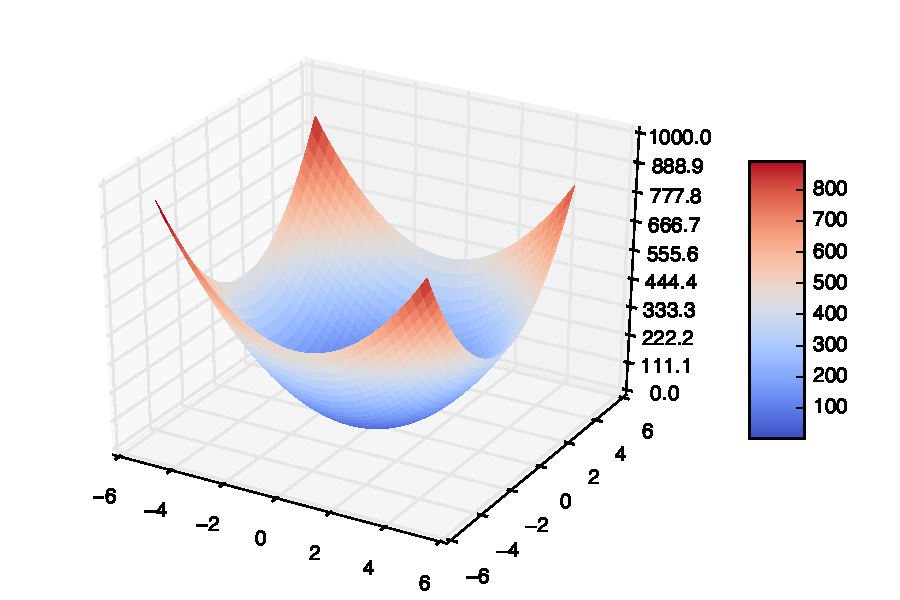
\includegraphics[scale = 0.34]{figures/localmin.pdf}

If $f$ is convex and finite near $x$, then either
\begin{itemize}
\item $x$ minimizes $f$, or
\item there is a descent direction for $f$ at $x$
\end{itemize}

\column{0.56\textwidth}
A quadratic function with a saddle point (index = 0): $x_1^2 - x_2^2 = y$
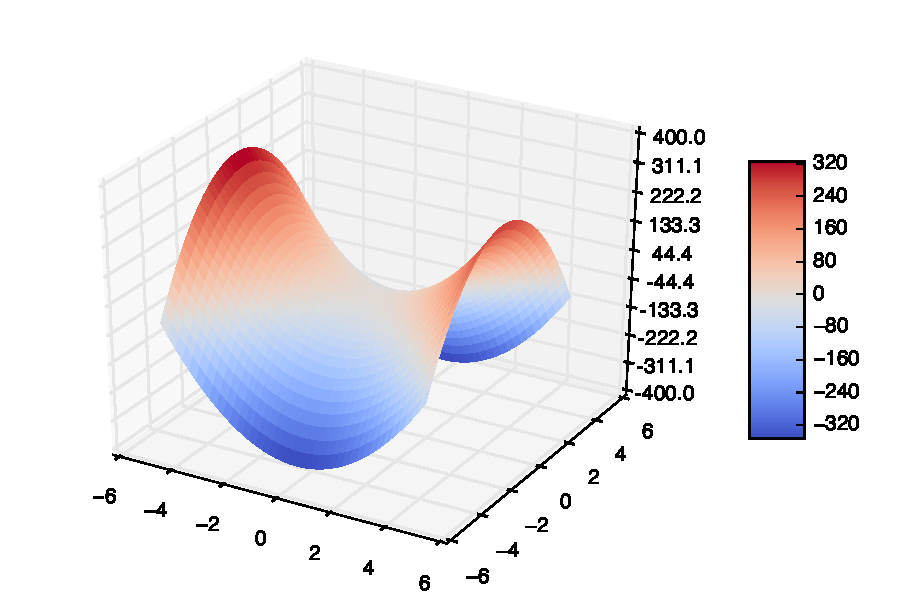
\includegraphics[scale = 0.34]{figures/saddle.pdf}

When does this theorem fail?
\begin{itemize}
\item Non-convex: saddles, valleys... 
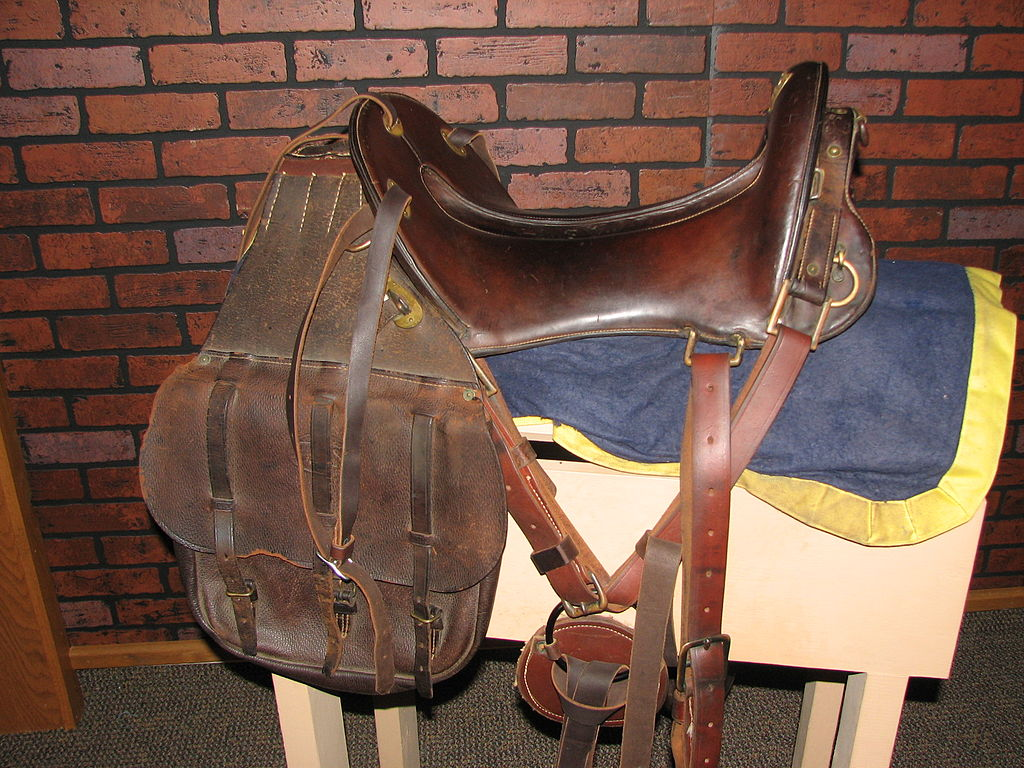
\includegraphics[scale = 0.12]{figures/1024px-McCellan_Saddle_Fort_Kearny_2006_C.jpg}
\vspace{3}
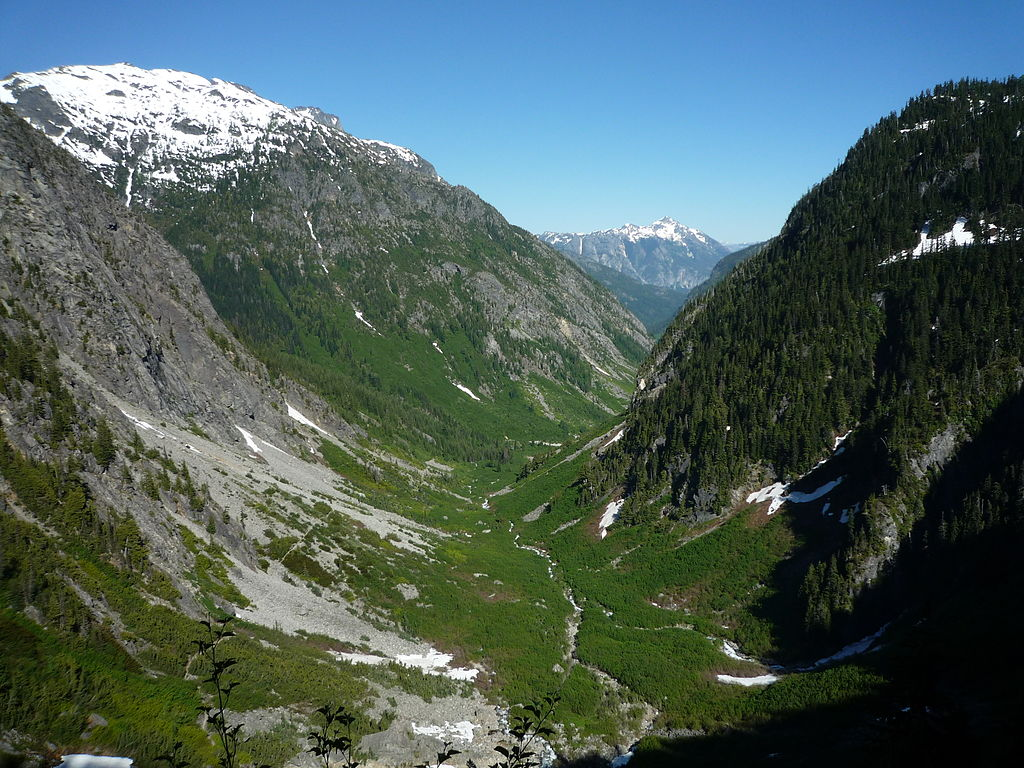
\includegraphics[scale = 0.12]{figures/1024px-Stehekin_River_Valley.jpg}
\item Unbounded
\end{itemize}

\end{columns}

\end{frame}

%---------------------------------------------------------

\begin{frame}
\frametitle{Directional derivative}
Let $f: \mathbb{R}^n \rightarrow \mathbb{R}$,
\begin{itemize}
    \item The gradient at any point of $\mathbb{R}^n$, is the best linear approximation to $f$ at that point. 
    \item For $f(x) = f(x_1,\dots, x_n)$, say we are given a unit vector $v=(v_1,\dots, v_n)$, then the directional derivative in the direction of $v$ is given by \[ \nabla_v f(x) = \lim_{h\rightarrow 0}\frac{f(x+hv)-f(x)}{h} \]
    \item This can be calculated using the gradient: $\nabla_v f(x) = \nabla f(x) \cdot v$
    \item It can be thought of the value of the rate of change in the direction $v$.
    \item Partial derivatives are special cases of this where the $v$ vector are unit coordinate vectors.
\end{itemize}


\end{frame}

%---------------------------------------------------------


\end{document}
